\section{Pipeline-Verarbeitung}
\label{sec:pipelining}

\textbf{Pipeline vs Seriell}
\begin{items}
  \item Seriell:
  \begin{figure}[ht]
    \centering
    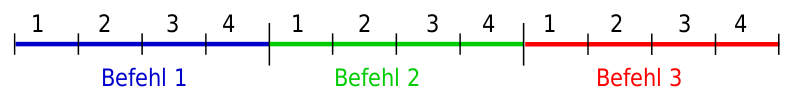
\includegraphics[width=0.33\textwidth]{Seriell}
    \label{Seriell}
  \end{figure}
  \item Pipelining:
  \begin{figure}[ht]
    \centering
    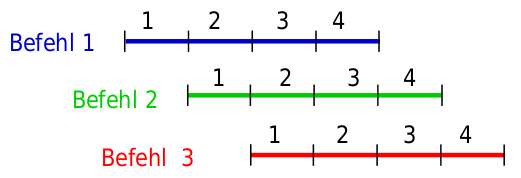
\includegraphics[width=0.33\textwidth]{Pipeline}
    \label{Pipeline}
  \end{figure}
\end{items}

\textbf{Beispiel: Wäsche waschen}
\begin{enumeration}
  \item Schmutzige Wäsche in Waschmaschine
  \item Nasse Wäsche in Trockner
  \item Falten/Bügeln
  \item Kleider in Schrank legen
\end{enumeration}
\begin{figure}[ht]
  \centering
  \label{PipelineWaesche}
  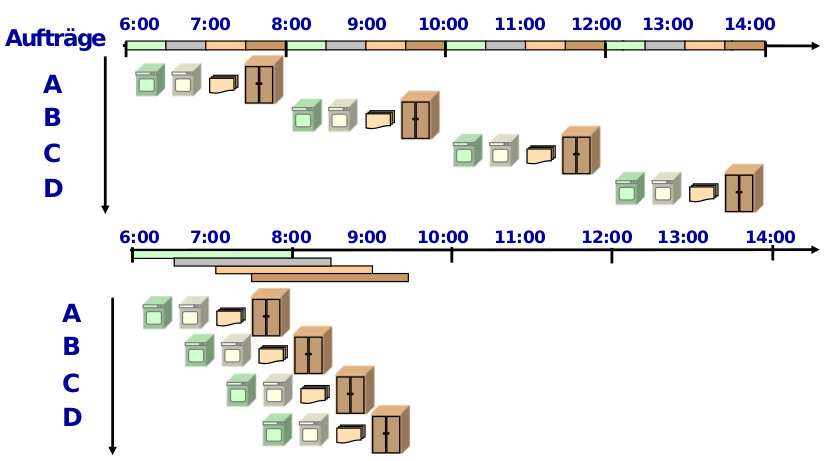
\includegraphics[width=0.33\textwidth]{PipelineWaesche}
\end{figure}

\textbf{Definition} \emph{Pipelining}: Operationszerlegung in mehrere Phasen/Suboperationen, die von hintereinandergeschalteten Verarbeitungseinheiten taktsynchron bearbeitet werden (jede Verarbeitungseinheit führt eine Teiloperation aus). \\*
$\leadsto$ Gesamtheit Verarbeitungseinheiten = Pipeline

\ \\

\textbf{Begrifflichkeiten}
\begin{items}
  \item \underline{Stufen, Register}:
  \begin{figure}[H]
    \centering
    \label{PipelineAufbau}
    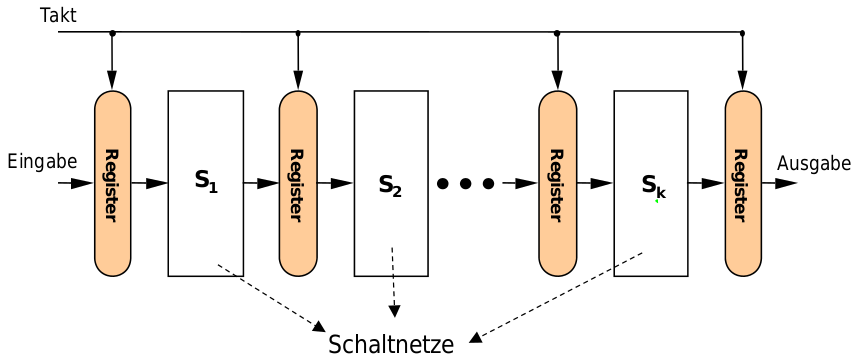
\includegraphics[width=0.33\textwidth]{PipelineAufbau}
  \end{figure}

  \item \underline{Verzögerungszeiten}: Schaltnetze: $\tau_i$ ($i=1,\dots,k$), Register: $\tau_{\text{reg}}$

  \item \underline{Pipeline-Maschinentakt}: Benötigte Zeit, um Befehl eine Stufe weiterzuschieben (ideal: $k$-stufige Pipeline führt Befehl in $k$ Takten mit $k$ Stufen aus)
  \item \underline{Latenz}: Zeit, die ein Befehl braucht, um alle $k$ Stufen zu durchlaufen
  \item \underline{Durchsatz}: Anzahl Befehle, die Pipeline pro Takt verlassen können: $D=\tfrac{n}{(k+n-1)*\tau}$ ($\tau: \text{max}\{ \tau_1,\dots,\tau_k \} + \tau_\text{reg}$) - $\lim_{n \to \infty} D = D_\text{max} = \tfrac{1}{\tau}$
  \item \underline{Speedup}: $n$ Befehle mit $k$-stufiger Pipeline ausführen:
  \begin{enumeration}
    \item sequentiell: $n*k$ Taktzyklen
    \item mit pipelining: $k+(n-1)$ Taktzyklen (Latenz $k$, Durchsatz $1$ - $k$ Takte zum Füllen, $(n-1)$ für die restlichen Befehle)
  \end{enumeration}
  $\leadsto$ Speedup $S=\tfrac{n*k}{k+n-1}$ (Leistungssteigerung - $\lim_{n \to \infty}S=k$)
\end{items}

\newpage

\textbf{MIPS  -- Befehlsabarbeitung}
\begin{items}
  \item \textbf{Befehl holen}: Wird bei jedem Befehlstyp benötigt
  \begin{enumeration}
    \item Befehl im Befehlsspeicher adressieren
    \item Befehlszähler (\code{PC}) um \( 4 \) inkrementieren
  \end{enumeration}
  \begin{figure}[H]\centering\label{BefehlHolen}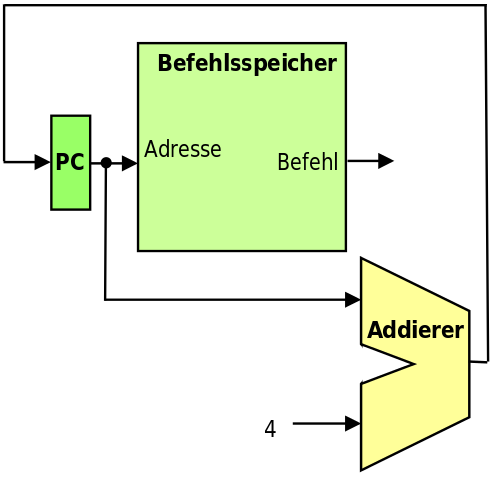
\includegraphics[width=0.2\textwidth]{BefehlHolen}\end{figure}

  \item \textbf{Typ R}: Lesezugriff auf beide Operandenregister, Schreibzugriff auf Zielregister
  \begin{figure}[H]\centering\label{Abarbeitung-R}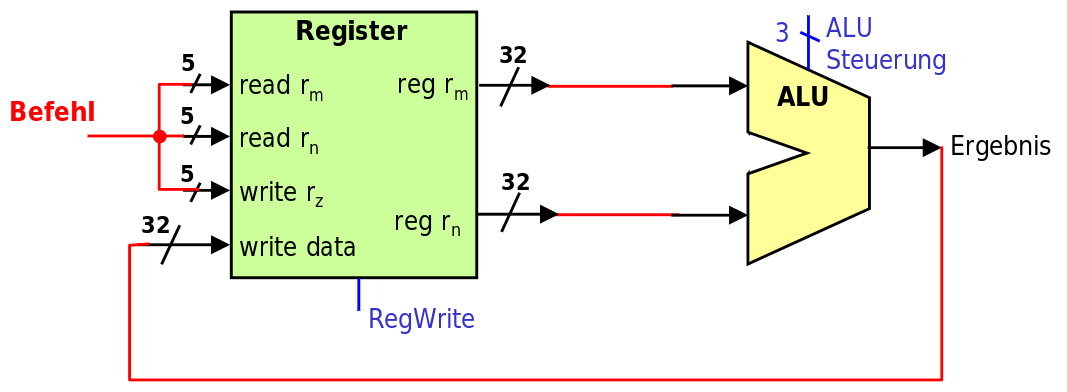
\includegraphics[width=0.33\textwidth]{Abarbeitung-R}\end{figure}

  \item \textbf{Typ I}: Bestimmung der Speicher-/Ladeadresse durch Addieren von 16-Bit-Offset zu Basisadresse in \( r_m \)
  \begin{enumeration}
    \item \underline{Laden} (z.B. \code{lw} \( r_z \)\code{, offset(}\( r_m \)\code{)}): Wort an Ladeadresse wird in \( r_z \) geladen
    \item \underline{Speichern} (z.B. \code{sw} \( r_n \)\code{, offset(}\( r_m \)\code{)}): Wort in \( r_n \) wird in Speicheradresse gespeichert
  \end{enumeration}
  \begin{figure}[H]\centering\label{Abarbeitung-I}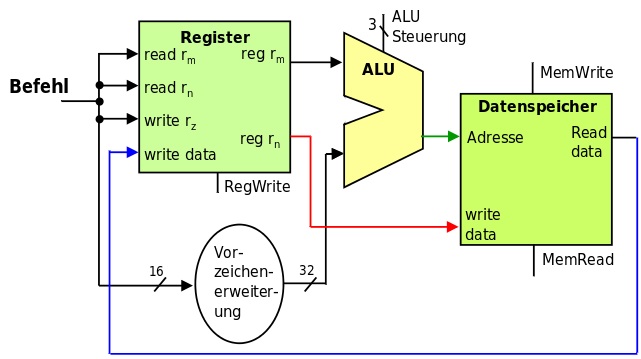
\includegraphics[width=0.33\textwidth]{Abarbeitung-I}\end{figure}

  \item \textbf{Typ J}: 16-Bit Offset \( \leadsto \) bis zu \( 2^{15}-1 \) Befehle vorwärts/\( 2^{15} \) rückwärts (Basisadresse zur Sprungberechnung = Befehlsadresse hinter Verzweigungsbefehl (\code{PC+4}), z.B. \code{beq} \( r_n, r_m \)\code{, offset}: Vergleich von \( r_n \), \( r_m \) entscheidet ob Sprung genommen wird)
  \begin{figure}[H]\centering\label{Abarbeitung-J}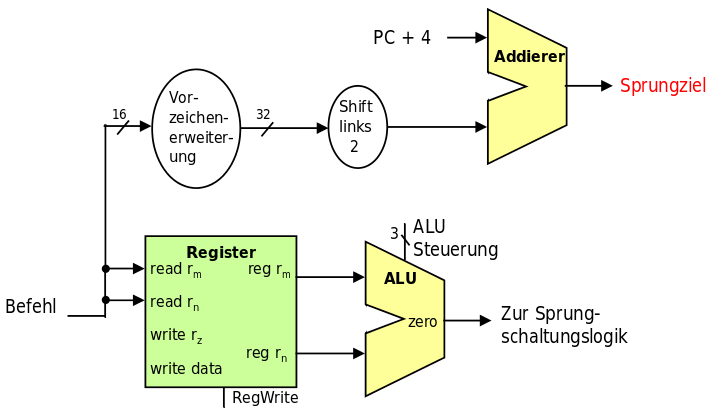
\includegraphics[width=0.33\textwidth]{Abarbeitung-J}\end{figure}

  \newpage

  \item \textbf{MIPS-Datenpfad}: Zusammenführung der drei Modelle
  \begin{figure}[H]\centering\label{MIPS-Datenpfad}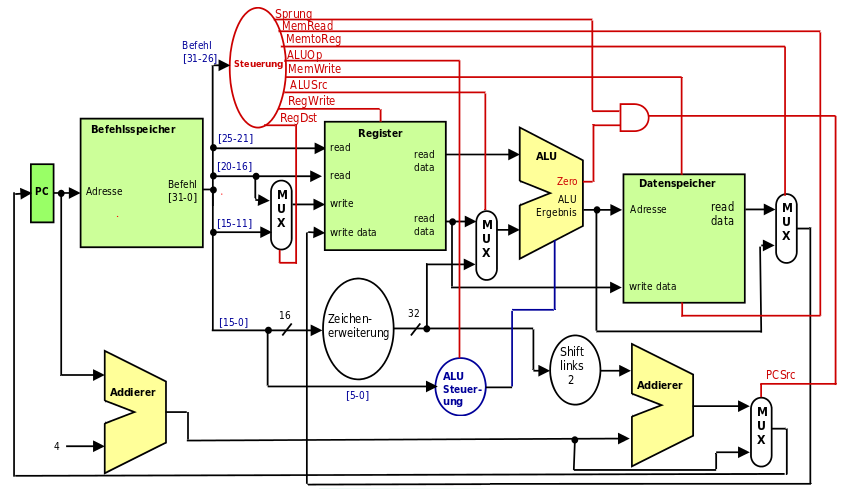
\includegraphics[width=0.5\textwidth]{MIPS-Datenpfad}\end{figure}
\end{items}

\textbf{MIPS -- Pipelining: DLX-Pipeline} (DLX = deluxe)
\begin{items}
  \item \textbf{Pipelinestufen, Buffering} (siehe Grafik "`Begrifflichkeiten: Stufen, Register"')
  \begin{figure}[H]\centering\label{MIPS-Buffering}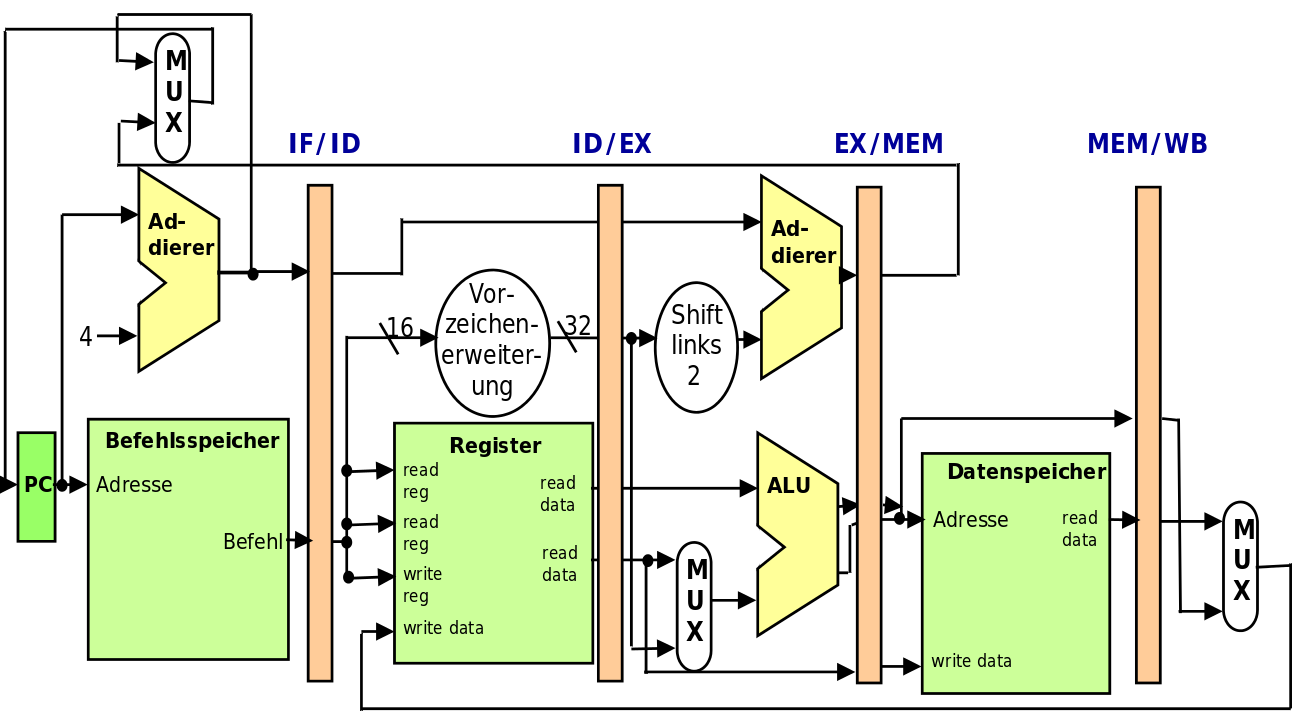
\includegraphics[width=0.5\textwidth]{MIPS-Buffering}\end{figure}
  \begin{enumeration}
    \item \underline{Phase 1 (\code{IF}-Phase)}: Instruction Fetch. Der durch Befehlszähler adressierte Befehl wird aus Cache/Speicher in Befehlsbuffer geladen, Befehlszähler wird inkrementiert
    \item \underline{Phase 2 (\code{ID/RF}-Phase)}: Instruktion Decode, Register Fetch. Aus Opcode werden prozessorinterne Steuersignale erzeugt, Operanden werden aus (Universal-)Register bereitgestellt
    \item \underline{Phase 3 (\code{EX}-Phase)}: Execution, Effective Address Calculation. Operation wird auf Operanden ausgeführt, bei Lade-/Speicherbefehl oder Verzweigung berechnet ALU effektive Adresse
    \item \underline{Phase 4 (\code{MEM}-Phase)}: Memory access. Speicherzugriff (bei Lade-/Speicherbefehl) wird durchfeführt
    \item \underline{Phase 5 (\code{WB}-Phase)}: Write back. Ergebnis wird in (Universal-)Register geschrieben (ergebnislose Befehle in dieser Phase passiv)
  \end{enumeration}
\end{items}

\newpage

\textbf{MIPS -- Pipeline-Konflikte}
\begin{items}
  \item \underline{Datenkonflikte}: Benötiger Operand ist in der Pipeline (noch) nicht verfügbar (Datenabhängigkeiten im Befehlsstrom)
  \item \underline{Struktur-/Ressourcenkonflikte}: Zwei Pipeline-Stufen benötigen selbe Ressource, aber nur einfacher Zugriff möglich
  \item \underline{Steuerflusskonflikte}: Bei Programmsteuerbefehlen
  \begin{enumeration}
    \item Zieladresse des nächsten Befehls in Befehlsbereitstellungsphase noch nicht berechnet
    \item Bedingter Sprung: noch unklar, ob gesprungen werden muss
  \end{enumeration}
\end{items}

\textbf{Datenabhängigkeiten/-konflikte}
\begin{items}
  \item \underline{Datenabhängigkeit}: Zwischen zwei aufeinanderfolgenden Befehlen \( Inst_1, Inst_2 \) kann eine \emph{Datenabhängigkeit} bestehen:
  \begin{enumeration}
    \item \textbf{Echte Datenabhängigkeit} (true dependence, \( \delta^t \)): \( Inst_1 \) schreibt Ausgabe in Register, dass die Eingabe von \( Inst_2 \) ist
    \item \textbf{Gegenabhängigkeit} (antidependence, \( \delta^a \)): \( Inst_1 \) liest von einer Stelle, die von \( Inst_2 \) überschrieben wird
    \item \textbf{Ausgabeabhängigkeit} (output dependence, \( \delta^o \)): \( Inst_1 \) und \( Inst_2 \) schreiben Ergebnis in selbes Register, aber \( Inst_2 \) nach \( Inst_1 \)
  \end{enumeration}

  \item \underline{Beispiel}:
  \begin{align*}
    S_1: \text{\code{add r1,r2,2}} &\quad \text{\code{# r1 := r2+2}} \\
    S_2: \text{\code{add r4,r1,r3}} &\quad \text{\code{# r4 := r1+r3}} \\
    S_3: \text{\code{mul r3,r5,3}} &\quad \text{\code{# r3 := r5*3}} \\
    S_4: \text{\code{mul r3,r6,3}} &\quad \text{\code{# r3 := r6*3}}
  \end{align*}
  \begin{figure}[H]\centering\label{Datenabhaengigkeiten}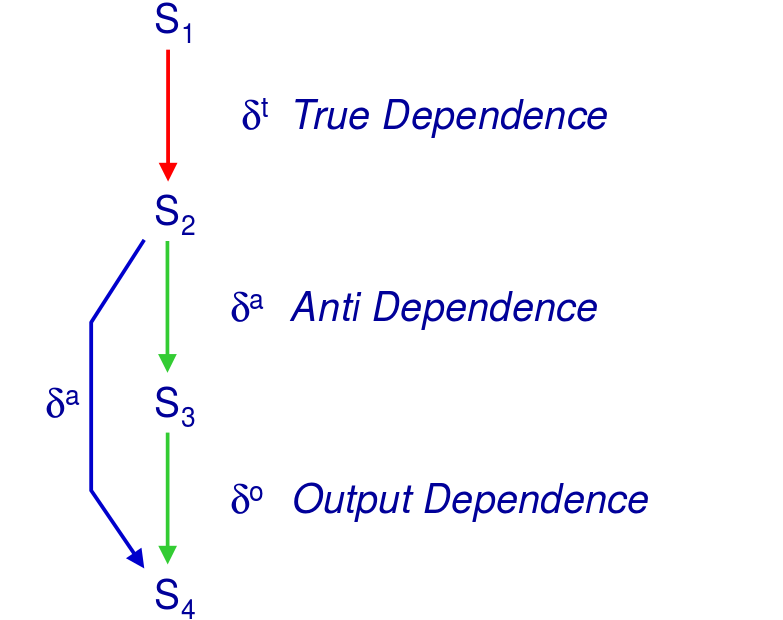
\includegraphics[width=0.2\textwidth]{Datenabhaengigkeiten}\end{figure}

  \item \underline{Datenkonflikte}:
  \begin{enumeration}
    \item \textbf{Lese-nach-Schreibe-Konflikt} (read after write, RAW): Verursacht durch echte Abhängigkeit
    \item \textbf{Schreibe-nach-Lese-Konflikt} (write after read, WAR): Verursacht durch Gegenabhängigkeit, tritt auf, wenn Schreib- vor Lesestufe in Pipeline
    \item \textbf{Schreibe-nach-Schreibe-Konflikt} (write after write, WAW): Verursacht durch Ausgabeabhängigkeit, tritt auf, wenn Pipeline in mehr als einer Stufe schreibt oder ein Befehl fortgesetzt werden darf, wenn vorhergehender angehalten wurde
  \end{enumeration}
  \item Kein WAR-/WAW-Konflikt in fünfstufiger DLX-Pipeline, da nicht überholt werden kann und immer in Stufe 2 gelesen wird (bzw. in Stufe 5 geschrieben)
  \item \underline{Lösungen}:
  \begin{enumeration}
    \item \textbf{Software-Lösung}: 
    \begin{enumeration}
      \item Compiler erkennt Datenkonflikte, fügt nach konfliktverursachenden Befehlen Leeroperation (\code{noop}) ein
      \item Statische Befehlsanordnung: Befehle werden umgeordnet (Optimierung), um Leeroperationen zu minimieren (Instruction Scheduling, Pipeline Scheduling)
    \end{enumeration}

    \newpage

    \item \textbf{Hardware-Lösung}:
    \begin{enumeration}
      \item Pipeline leerlaufen lassen: Pipeline-Sperrung (\emph{interlocking}) bzw. Pipeline-Leerlauf (\emph{stalling})
      \begin{figure}[H]\centering\label{Interlocking}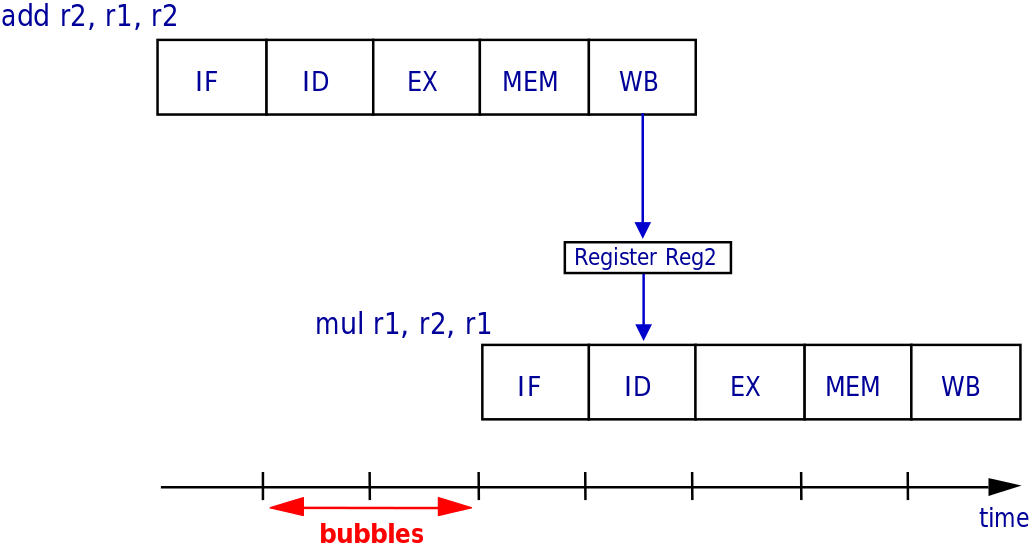
\includegraphics[width=0.33\textwidth]{Interlocking}\end{figure}
      \item \emph{Forwarding}: Wird Datenkonflikt erkannt, so wird Operand nicht aus Universalregister, sondern direkt aus ALU-Ausgaberegister der vorherigen Operation in ALU-Eingaberegister übertragen
      \begin{figure}[H]\centering\label{Forwarding}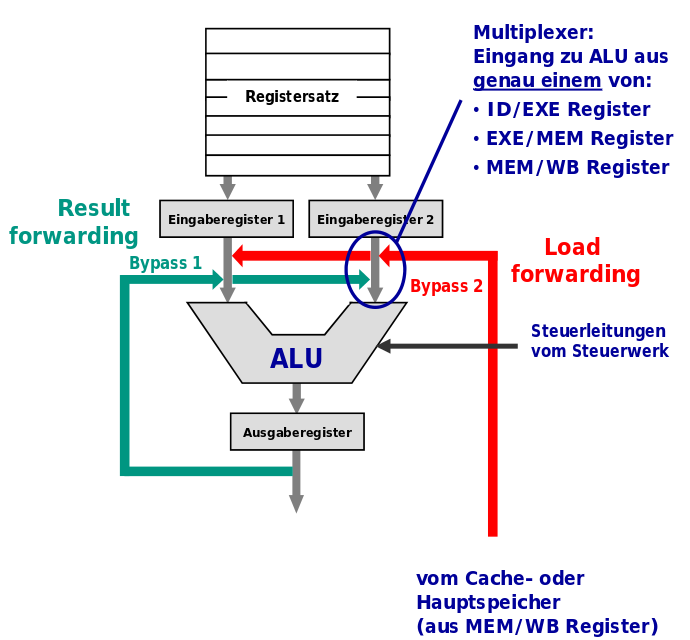
\includegraphics[width=0.33\textwidth]{Forwarding}\end{figure}
      \item \emph{Forwarding with interlocking}: Forwarding löst nicht alle möglichen Datenkonflikte
      \begin{figure}[H]\centering\label{ForwardingInterlocking}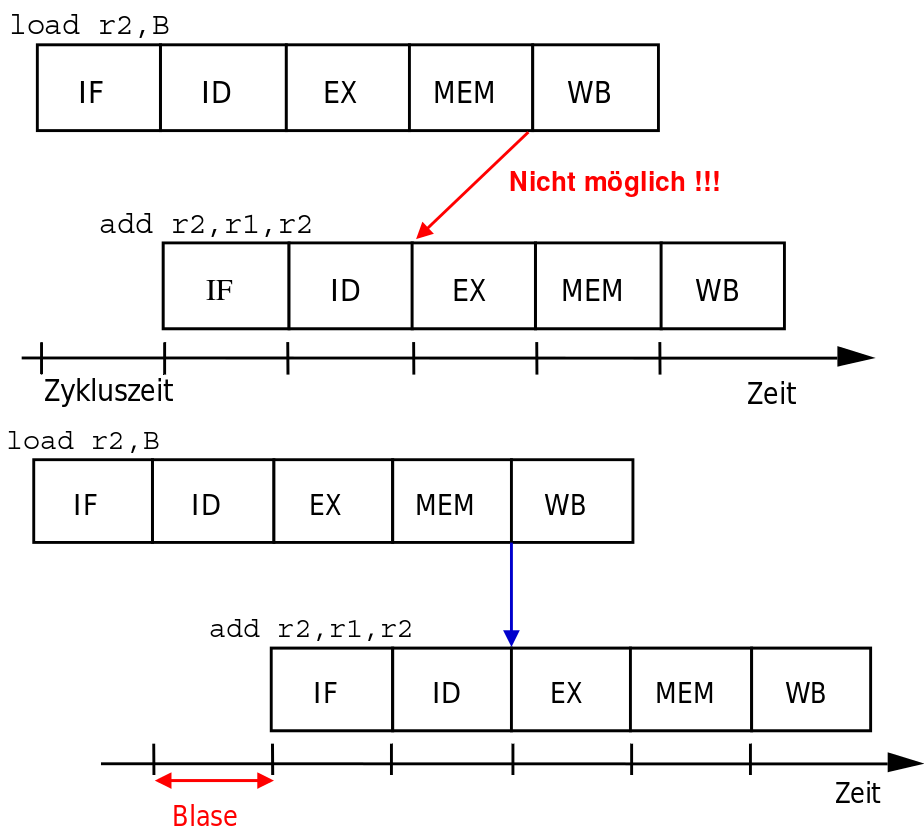
\includegraphics[width=0.33\textwidth]{ForwardingInterlocking}\end{figure}
    \end{enumeration}
  \end{enumeration}
\end{items}

\textbf{Ressourcenkonflikte}
\begin{items}
  \item Treten bei einfachen Modellen wie einer DLX-Pipeline nicht auf
  \item \underline{Lösungen}:
  \begin{enumeration}
    \item \textbf{Arbitrierung mit Interlocking}: Arbitrierungslogik hält konfliktverursachenden Befehl an \( \leadsto \) Verzögerung
    \item \textbf{Übertaktung}: Konfliktverursachende Ressource wird schneller getaktet als übrige Pipeline-Stufen
    \item \textbf{Ressourcenreplizierung}: Ressourcen werden vervielfacht (z.B. Registersatz mit mehreren Schreibkanälen) 
  \end{enumeration}
\end{items}

\newpage

\textbf{Steuerflusskonflikte}
\begin{items}
  \item \underline{Programmsteuerbefehle}: bedingte und unbedingte Sprünge, Unterprogrammaufruf- und -rückkehrbefehle, Unterbrechungsbefehle
  \item Befehlszähler wird erst in \code{MEM}-Stufe ersetzt \( \leadsto \) Befehle in Pipeline, die wieder gelöscht werden müssen
  \begin{figure}[H]\centering\label{Steuerflusskonflikt}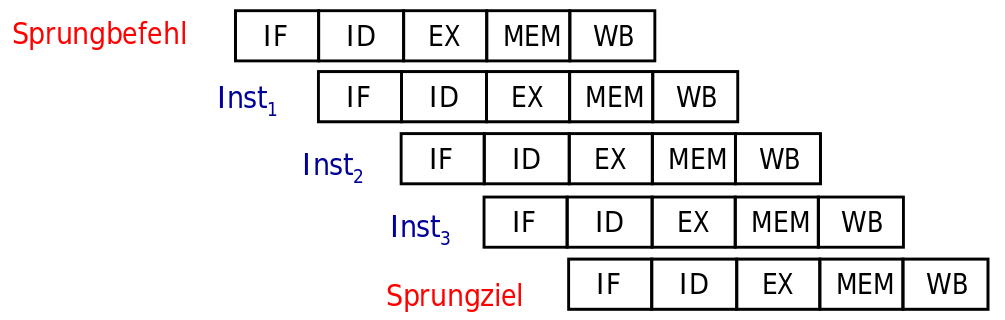
\includegraphics[width=0.33\textwidth]{Steuerflusskonflikt}\end{figure}
  \item \( \leadsto \) nach genommenem Sprung müssen Wartezyklen eingefügt werden (die ggf. durch Umstrukturierung der Pipeline verringert werden können)
  \begin{figure}[H]\centering\label{Pipeline-Wartezyklen}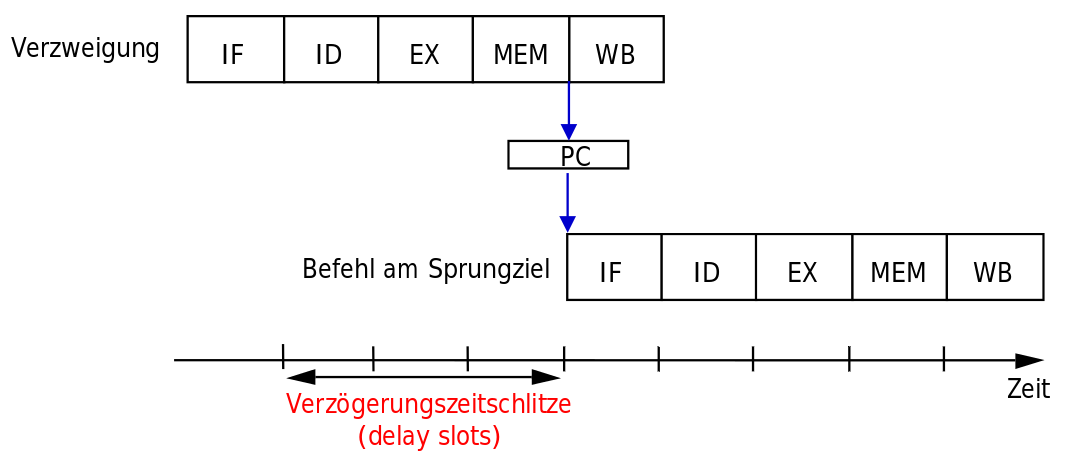
\includegraphics[width=0.33\textwidth]{Pipeline-Wartezyklen}\end{figure}

  \item \underline{Lösungen}:
  \begin{enumeration}
    \item \textbf{Software-Lösung}:
    \begin{enumeration}
      \item Einfügen von \code{noop} in die Wartezyklen
      \item Statische Befehlsanordnung: Compiler optimiert Code und fügt nicht sprungrelevante Befehle in Wartezyklen ein, \code{noop}, falls es keine gibt \( \leadsto \) Code Pipeline-abhängig
    \end{enumeration}
    \item \textbf{Hardware-Lösung}:
    \begin{enumeration}
      \item Hardware Erkennt Verzweigungsbefehle in ID-Stufe und lädt danach bis zur Berechnung der Zieladresse keine weiteren Befehle \( \leadsto \) bereits in \code{IF}-Stufe geladener Befehl muss gelöscht werden
      \item Spekulation auf nicht genommene bedingte Sprünge - wird Sprung doch genommen Pipeline leeren (\emph{Pipeline flushing})
      \item 1-Bit-Prädikator zur Sprungvorhersage
      \begin{figure}[H]\centering\label{1-Bit-Praediktor}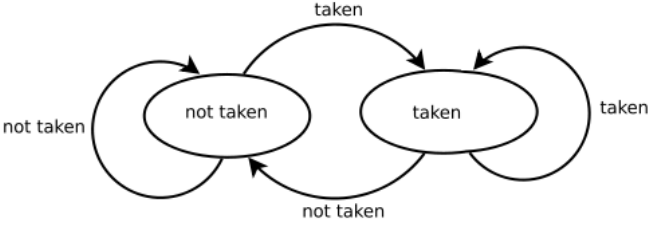
\includegraphics[width=0.33\textwidth]{1-Bit-Praediktor}\end{figure}
      \item 2-Bit-Prädiktor zur Sprungvorhersage
      \begin{figure}[H]\centering\label{2-Bit-Praediktor}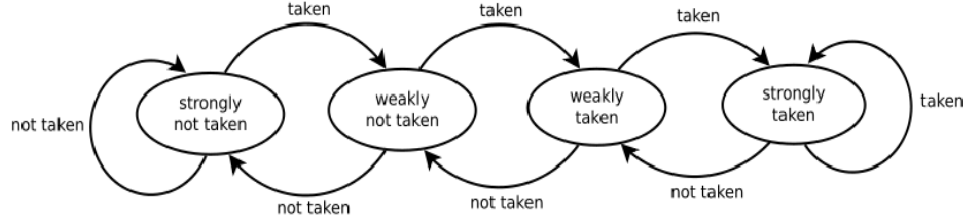
\includegraphics[width=0.33\textwidth]{2-Bit-Praediktor}\end{figure}
      \item Moderne Sprungvorhersagetechniken: In mehr als \( 90\% \) der Fälle richtig
    \end{enumeration}
  \end{enumeration}
\end{items}